
\chapter{Dạng bài: Vẽ ảnh tạo bởi thấu kính }

	
\section{Kiến thức cần nhớ}
\subsection{ Đường truyền của tia sáng qua thấu kính thấu kính hội tụ}
\begin{itemize}
	\item Tia tới đi qua quang tâm O thì cho tia ló tiếp tục truyền thẳng.
	\begin{center}
		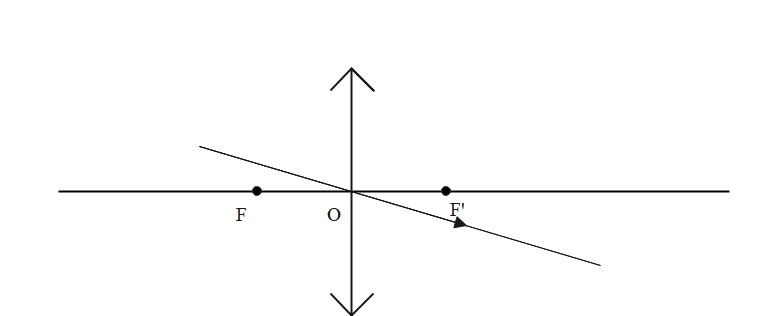
\includegraphics[scale=0.7]{../figs/VN11-PH-38-A-004-1-h19.jpg}
	\end{center}
	\item Tia tới song song trục chính thì cho tia ló qua tiêu điểm ảnh chính F'.
	\begin{center}
		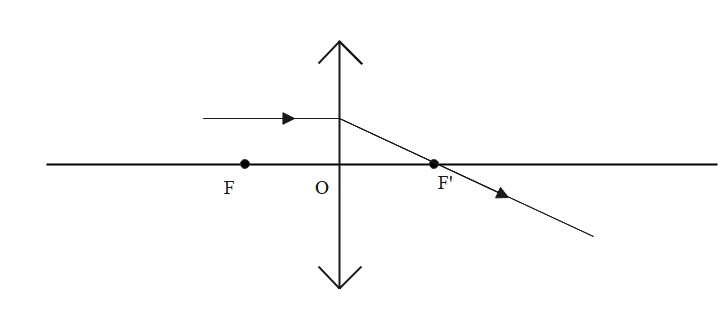
\includegraphics[scale=0.7]{../figs/VN11-PH-38-A-004-1-h20.jpg}
	\end{center}
	\item Tia tới đi qua tiêu điểm vật chính F thì cho tia ló song song trục chính. 
	\begin{center}
		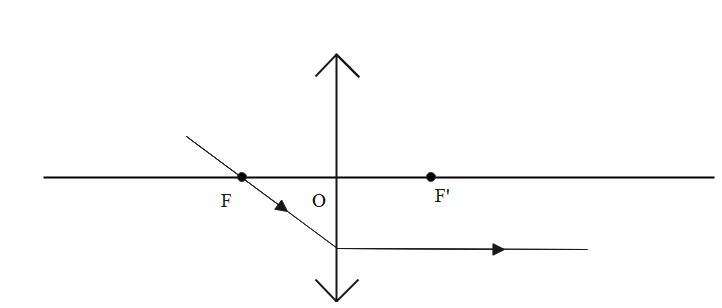
\includegraphics[scale=0.7]{../figs/VN11-PH-38-A-004-1-h21.jpg}
	\end{center}
\end{itemize}
\subsection{ Đường truyền của tia sáng qua thấu  kính thấu kính phân kỳ}
\begin{itemize}
	\item Tia tới đi qua quang tâm O thì cho tia ló tiếp tục truyền thẳng.
	\begin{center}
		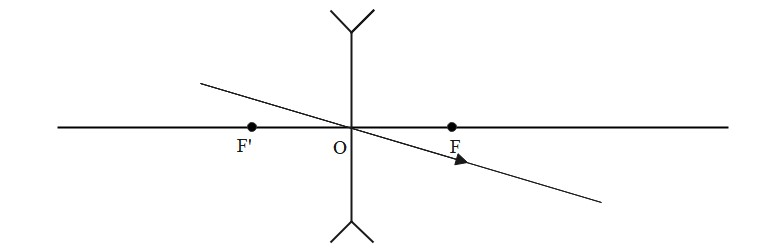
\includegraphics[scale=0.7]{../figs/VN11-PH-38-A-004-1-h22.jpg}
	\end{center}
	\item Tia tới song song trục chính thì cho tia ló có đường kéo dài qua tiêu điểm ảnh chính F'.
	\begin{center}
		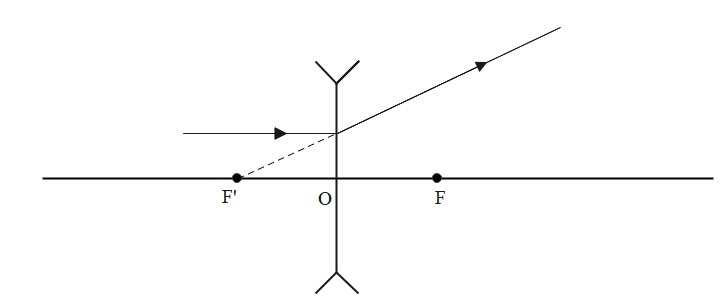
\includegraphics[scale=0.7]{../figs/VN11-PH-38-A-004-1-h23.jpg}
	\end{center}
	\item Tia tới có đường kéo dài đi qua tiêu điểm vật chính F thì cho tia ló song song trục chính.
	\begin{center}
		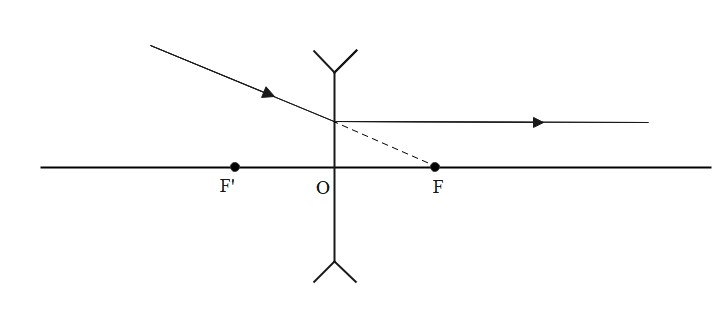
\includegraphics[scale=0.7]{../figs/VN11-PH-38-A-004-1-h24.jpg}
	\end{center} 
\end{itemize}
\subsection{Cách dựng ảnh tạo bởi thấu kính}
Vẽ đường đi của hai trong số các tia tới đặc biệt sau:
\begin{itemize}
	\item Tia tới qua quang tâm O thì tia ló tiếp tục truyền thẳng.
	\item Tia tới song song với trục chính của thấu kính. thì tia ló (hoặc đường kéo dài của tia ló) sẽ đi qua tiêu điểm ảnh chính.
	\item Tia tới qua tiêu điểm vật chính F (hay có đường kéo dài qua F) thì tia ló sẽ song song với trục chính.
\end{itemize}
Giao điểm của các tia ló (hoặc đường kéo dài các tia ló) chính là vị trí của ảnh. 
\begin{center}
	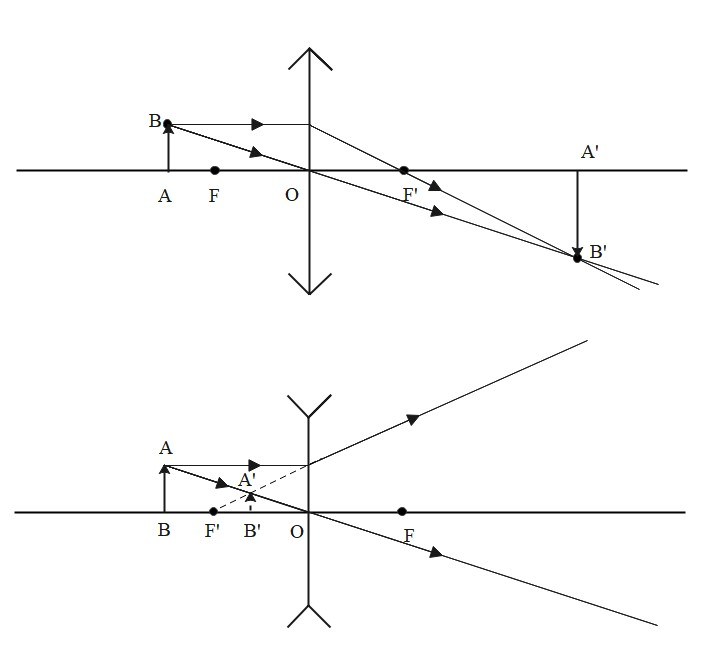
\includegraphics[scale=0.7]{../figs/VN11-PH-38-A-004-1-h25.jpg}
\end{center}
Trường hợp tia sáng bất kỳ thì cách xác định tia ló như sau:
\begin{itemize}
	\item Dựng trục phụ song song với tia tới.
	\item Từ F' dựng đường thẳng vuông góc  với trục chính, cắt trục phụ tại $\text{F'}_1$.
	\item Nối điểm tới I và $\text{F'}_1$ ta được tia ló.
	\begin{center}
		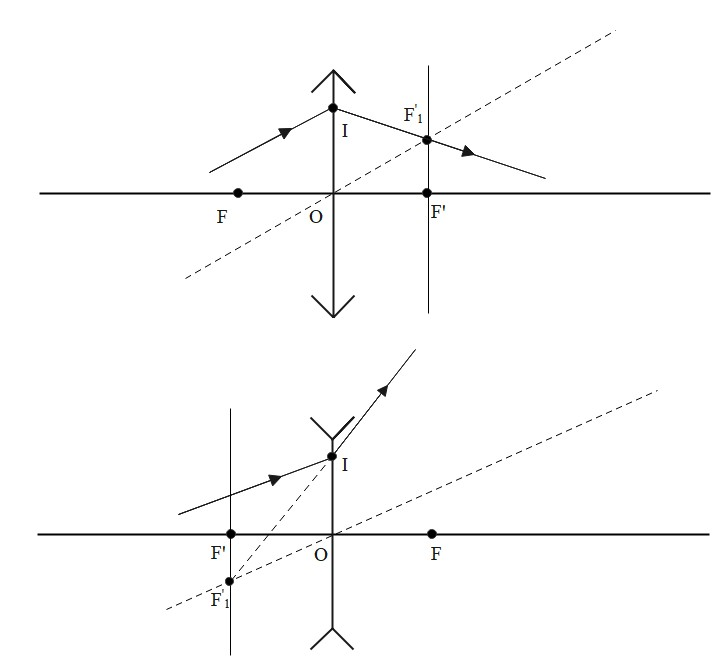
\includegraphics[scale=0.7]{../figs/VN11-PH-38-A-004-1-h26.jpg}
	\end{center} 
	
\end{itemize}
\section{Phương pháp giải}
		\textbf{Nếu đề bài cho điểm sáng S nằm ngoài trục chính. Yêu cầu xác định điểm ảnh S'.}
		\begin{description}
		
					\item[Bước 1:] Từ S, ta vẽ tia tới đi qua quang tâm cho tia ló truyền thẳng.
					\item[Bước 2:] Từ S, ta vẽ tia tới song song với trục chính cho tia ló đi qua tiêu điểm F'.
					\item[Bước 3:] Giao điểm giữa hai tia ló chính là ảnh S' của S tạo bởi thấu kính.
\end{description}

			\textbf{Nếu đề bài cho vật sáng AB. Yêu cầu xác định ảnh A'B'.}
			
			Muốn dựng ảnh của một vật sáng AB có dạng mũi tên, A nằm trên trục chính ta chỉ cần dựng ảnh của điểm sáng B.
			\begin{description}
						\item[Bước 1:] Từ B, ta vẽ tia tới đi qua quang tâm cho tia ló truyền thẳng. 				
					\item[Bước 2:] Từ B, ta vẽ tia tới song song với trục chính cho tia ló đi qua tiêu điểm F'.
					\item[Bước 3:] Giao điểm giữa hai tia ló chính là ảnh B' của B tạo bởi thấu kính.
					\item[Bước 4:] Từ B dựng A'B' vuông góc với trục chính A (A' là ảnh của A). Khi đó A'B' là ảnh của AB.
			
	\end{description}
		
			\luuy{
			\begin{itemize}
				\item	\textbf{Nếu đề bài cho vật điểm S và ảnh điểm S'}, trục chính thì S và S' cắt nhau tại quang tâm O trên trục chính. Dựa vào vị trí của S,S' so với trục chính ta kết luận được S’ là ảnh thật hay ảo, thấu kính là hội tụ hay phân kì.
				\item \textbf{Nếu đề bài cho vật AB và ảnh A'B'}, tiến hành nối AB và A'B' chúng cắt nhau tại quang tâm O, Ox vuông góc với AB sẽ là trục chính của thấu kính. 
				\item \textbf{Xác định tiêu điểm F:} Từ S hoặc AB vẽ tia SI song song  trục chính, giao trục chính với IS’ là F.
				\end{itemize}
	
	}
\section{Ví dụ minh họa}
\viduii{2}{
Vẽ ảnh của điểm sáng S trong các trường hợp sau và cho biết tính chất ảnh. 

		Câu a.
		
		\begin{center}
			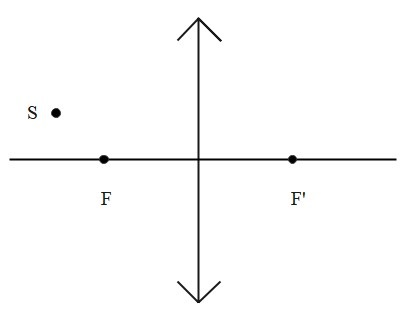
\includegraphics[scale=0.7]{../figs/VN11-PH-38-A-004-1-h8.jpg}
		\end{center}
	
		Câu b. 
		\begin{center}
			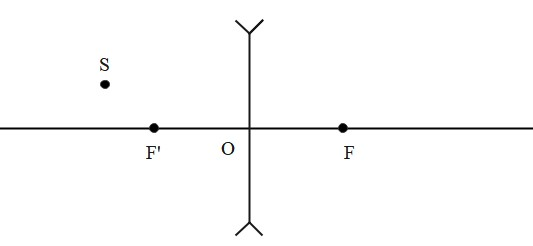
\includegraphics[scale=0.7]{../figs/VN11-PH-38-A-004-1-h9.jpg}
		\end{center}
	}
{

\begin{center}
	\textbf{Hướng dẫn giải:}
\end{center}
	
	{
			Câu a. 
			\begin{itemize}
				
		\item Từ S, ta vẽ tia tới đi qua quang tâm cho tia ló truyền thẳng.
		\item Từ S, ta vẽ tia tới song song với trục chính cho tía ló đi qua tiêu điểm F'.
		\item  Giao điểm giữa hai tia ló chính là ảnh S' của S tạo bởi thấu kính.
		
		Ảnh S' là ảnh thật, ảnh và vật nằm khác phía so với trục chính, ảnh nằm xa thấu kính hơn vật.
			\end{itemize}
		\begin{center}
			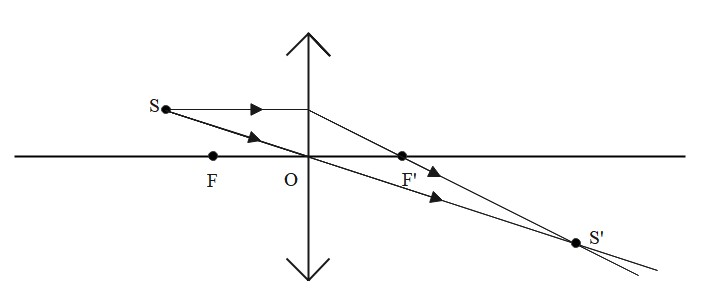
\includegraphics[scale=0.7]{../figs/VN11-PH-38-A-004-1-h10.jpg}
		\end{center}
		Câu b. 
			\begin{itemize}
		\item Từ S, ta cũng vẽ tia tới đi qua quang tâm cho tia ló truyền thẳng.
		\item Từ S, ta vẽ tia tới song song với trục chính cho tía ló đi qua tiêu điểm F'.
		\item  Giao điểm giữa hai tia ló chính là ảnh S' của S tạo bởi thấu kính.
		
		Ảnh S' là ảnh ảo, ảnh và vật nằm cùng phía so với trục chính, ảnh nằm gần thấu kính hơn vật.
		
			\end{itemize}
		\begin{center}
			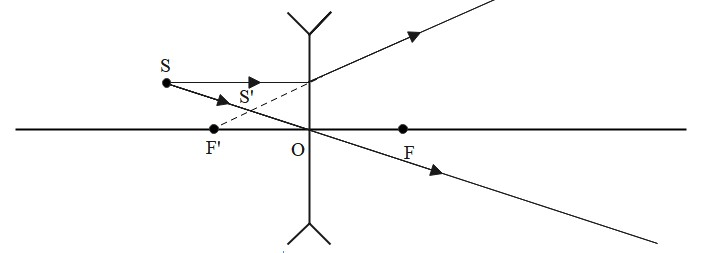
\includegraphics[scale=0.7]{../figs/VN11-PH-38-A-004-1-h11.jpg}
		\end{center}
			}
}
\viduii{2}{
Vẽ ảnh của vật sáng AB  trong các trường hợp sau và cho biết tính chất ảnh. 

Câu a.

\begin{center}
	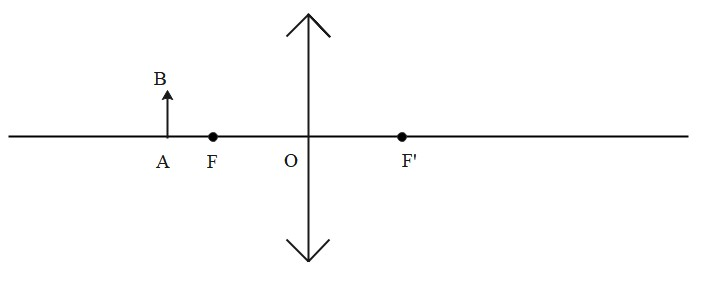
\includegraphics[scale=0.7]{../figs/VN11-PH-38-A-004-1-h12.jpg}
\end{center}

Câu b. 
\begin{center}
	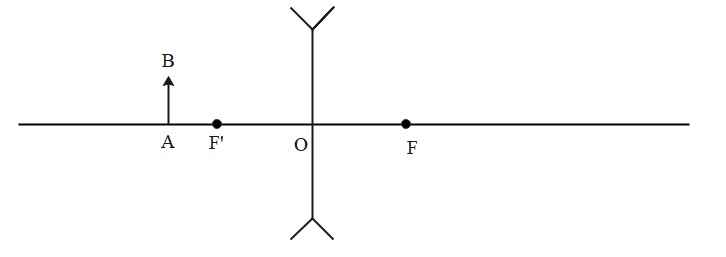
\includegraphics[scale=0.7]{../figs/VN11-PH-38-A-004-1-h13.jpg}
\end{center}

}
{\begin{center}
	\textbf{Hướng dẫn giải:}
\end{center}

	Câu a. 
	\begin{itemize}
		\item Từ B, ta vẽ tia tới đi qua quang tâm cho tia ló truyền thẳng. 
		\item Từ B, ta vẽ tia tới song song với trục chính cho tia ló đi qua tiêu điểm F'.
		\item  Giao điểm giữa hai tia ló chính là ảnh B' của B tạo bởi thấu kính.
		\item Từ B dựng A'B' vuông góc với trục chính A (A' là ảnh của A). Khi đó A'B' là ảnh của AB.
		
		Ảnh A'B' là ảnh thật, ngược chiều vật, lớn hơn vật.
	\end{itemize}
	\begin{center}
		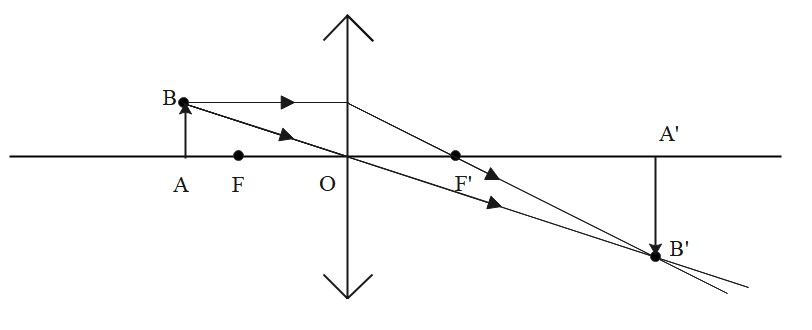
\includegraphics[scale=0.7]{../figs/VN11-PH-38-A-004-1-h14.jpg}
	\end{center}
	Câu b. 
	\begin{itemize}
	\item Từ B, ta vẽ tia tới đi qua quang tâm cho tia ló truyền thẳng. 
	\item Từ B, ta vẽ tia tới song song với trục chính cho tia ló có đường kéo dài đi qua tiêu điểm F'.
	\item  Giao điểm giữa hai tia ló chính là ảnh B' của B tạo bởi thấu kính.
	\item Từ B dựng A'B' vuông góc với trục chính A (A' là ảnh của A). Khi đó A'B' là ảnh của AB.
	
	Ảnh A'B' là ảnh ảo, cùng chiều vật,nhỏ hơn vật.
	\end{itemize}
	\begin{center}
		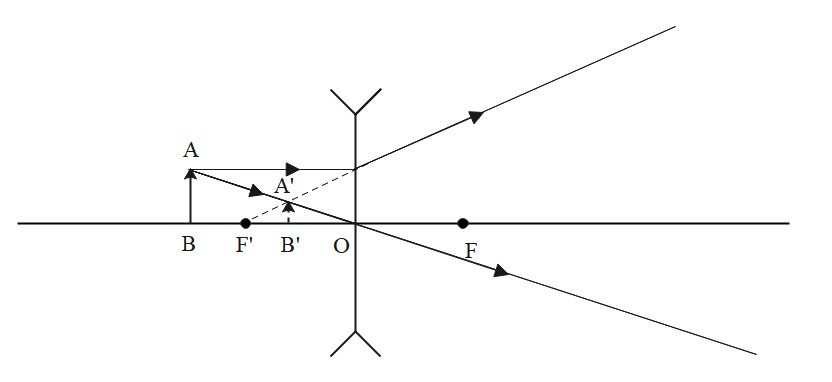
\includegraphics[scale=0.7]{../figs/VN11-PH-38-A-004-1-h15.jpg}
	\end{center}
}
\viduii{3}{Cho A là vật điểm , A' là ảnh điểm. Xác định: tính chất ảnh, loại thấu kính, vị trí tiêu điểm F và F'.
\begin{center}
	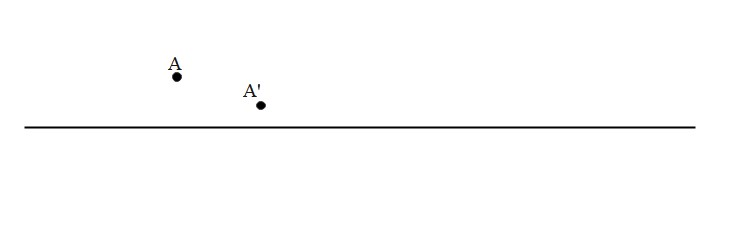
\includegraphics[scale=0.7]{../figs/VN11-PH-38-A-004-1-h16.jpg}
\end{center}
}{
\begin{center}
	\textbf{Hướng dẫn giải:}
\end{center}

{		\begin{itemize}
		
		\item Vì ảnh A và A' nằm cùng phía so với trục chính nên A và A' trái tính  chất nhau, suy ra A' là ảnh ảo.
		\item 	Vì khoảng cách từ A' đến trục chính nhỏ hơn khoảng cách từ A đến trục chính nên ảnh ảo nhỏ hơn vật, suy ra thấu kính là thấu kính phân kỳ.
		\item  	Vẽ hình:
		\begin{itemize}
		\item  	Vì điểm vật A, ảnh A' và quang tâm O thẳng hàng nên AA' cắt trục chính tại quang tâm O.
		
			\item  Qua O dựng thấu kính phân kỳ vuông góc với trục chính.
			\item  Kẻ tia tới AI song song với trục chính thì tia ló qua I có đường kéo dài qua A', cắt trục chính tại tiêu điểm F'. 
			\item  Lấy F đối xứng với F' qua O, ta tìm được tiêu điểm F.
			\end{itemize}
	\end{itemize}
		\begin{center}
		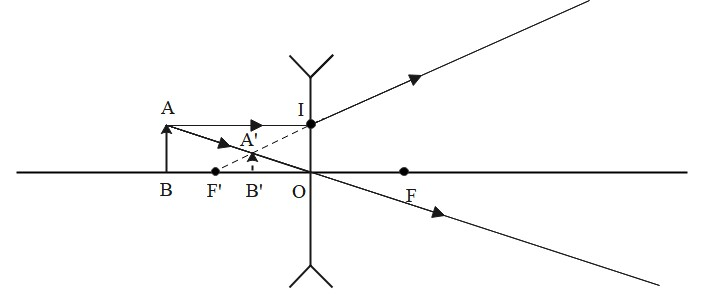
\includegraphics[scale=0.7]{../figs/VN11-PH-38-A-004-1-h27.jpg}
	\end{center}

}
}

